%  LaTeX support: latex@mdpi.com
%  In case you need support, please attach any log files that you could have, and specify the details of your LaTeX setup (which operating system and LaTeX version / tools you are using).

%=================================================================

% LaTeX Class File and Rendering Mode (choose one)
% You will need to save the "mdpi.cls" and "mdpi.bst" files into the same folder as this template file.

%=================================================================

\documentclass[atoms,article,submit,moreauthors,dvi2pdf,12pt,a4paper]{mdpi}
%--------------------
% Class Options:
%--------------------
% journal
%----------
% Choose between the following MDPI journals:
% actuators, administrativesciences, aerospace, agriculture, agronomy, algorithms, animals, antibiotics, antibodies, antioxidants, appliedsciences, arts, atmosphere, atoms, axioms, batteries, behavioralsciences, bioengineering, biology, biomedicines, biomolecules, biosensors, brainsciences, buildings, cancers, catalysts, cells, challenges, chemosensors, children, chromatography, climate, coatings, computation, computers, cosmetics, crystals, dentistryjournal, diagnostics, diseases, diversity, econometrics, economies, education, electronics, energies, entropy, environmentalsciences, environments, epigenomes, fibers, foods, forests, futureinternet, gvalaxies, games, gels, genealogy, genes, geosciences, healthcare, horticulturae, humanities, hydrology, informatics, information, inorganics, insects, ijerph, ijfs, ijms, ijgi, jcdd, jcm, jdb, jfb, jimaging, jof, joi, jlpea, jmse, jpm, jrfm, jsan, land, laws, life, lubricants, machines, marinedrugs, materials, mathematics, medicalsciences, membranes, metabolites, metals, microarrays, micromachines, microorganisms, minerals, molbank, molecules, nanomaterials, ncrna, nutrients, pathogens, pharmaceuticals, pharmaceutics, pharmacy, photonics, plants, polymers, processes, proteomes, publications, religions, remotesensing, resources, risks, robotics, safety, sensors, sinusitis, socialsciences, societies, sports, standards, sustainability, symmetry, systems, technologies, toxics, toxins, universe, vaccines, veterinarysciences, viruses, water
%---------
% article
%---------
% The default type of manuscript is article, but could be replaced by using one of the class options:
% article, review, communication, commentary, bookreview, correction, addendum, editorial, changes, supfile, casereport, comment, conceptpaper, conferencereport, meetingreport, discussion, essay, letter, newbookreceived, opinion, projectreport, reply, retraction, shortnote, technicalnote, creative
%----------
% submit
%----------
% The class option "submit" will be changed to "accept" by the Editorial Office when the paper is accepted. This will only make changes to the frontpage (e.g. the logo of the journal will get visible), the headings, and the copyright information. Journal info and pagination for accepted papers will also be assigned by the Editorial Office.
% Please insert a blank line is before and after all equation and eqnarray environments to ensure proper line numbering when option submit is chosen
%------------------
% moreauthors
%------------------
% If there is only one author the class option oneauthor should be used. Otherwise use the class option moreauthors.
%---------
% pdftex
%---------
% The option "pdftex" is for use with pdfLaTeX only. If eps figure are used, use the optioin "dvipdfm", with LaTeX and dvi2pdf only.

%=================================================================
\setcounter{page}{1}
\lastpage{x}
\doinum{10.3390/------}
\pubvolume{xx}
\pubyear{2015}
%\externaleditor{Academic Editor: xx}
\history{Received: xx / Accepted: xx / Published: xx}
%------------------------------------------------------------------
% The following line should be uncommented if the LaTeX file is uploaded to arXiv.org
%\pdfoutput=1

%=================================================================

% Add packages and commands to include here
% The amsmath, amsthm, amssymb, hyperref, caption, float and color packages are loaded by the MDPI class.
\usepackage{graphicx}
\usepackage{color}
\usepackage{verbatim}
%\usepackage{subfigure,psfig}

%=================================================================
%% Please use the following mathematics environments:
%\theoremstyle{mdpi}
%\newcounter{thm}
%\setcounter{thm}{0}
%\newcounter{ex}
%\setcounter{ex}{0}
%\newcounter{re}
%\setcounter{re}{0}
%\newtheorem{Theorem}[thm]{Theorem}
%\newtheorem{Lemma}[thm]{Lemma}
%\newtheorem{Characterization}[thm]{Characterization}
%\newtheorem{Proposition}[thm]{Proposition}
%\newtheorem{Property}[thm]{Property}
%\newtheorem{Problem}[thm]{Problem}
%\newtheorem{Example}[ex]{Example}
%\newtheorem{Remark}[re]{Remark}
%\newtheorem{Corollary}[thm]{Corollary}
%\newtheorem{Definition}[thm]{Definition}
%% For proofs, please use the proof environment (the amsthm package is loaded by the MDPI class).

%=================================================================
\def\be{\begin{equation}}
\def\ee{\end{equation}}
\def\ba{\begin{eqnarray}}
\def\ea{\end{eqnarray}}
% Full title of the paper (Capitalized)
\Title{Photon-Induced Spin-Orbit Coupling in Ultracold Atoms inside Optical Cavity}

% Authors (Add full first names)
\Author{Lin Dong $^{1,}$, Chuanzhou Zhu $^{1}$ and Han Pu $^{1,2}$*}

% Affiliations / Addresses (Add [1] after \address if there is only one affiliation.)
\address{%
$^{1}$ Department of Physics and Astronomy, Rice Quantum Institute, Rice University, Houston, Texas, 77251-1892, USA \\
$^{2}$ Center for Cold Atom Physics, Chinese Academy of Sciences, Wuhan 430071, China
}


% Contact information of the corresponding author (Add [2] after \corres if there are more than one corresponding author.)
\corres{hpu@rice.edu}

% Abstract (Do not use inserted blank lines, i.e. \\)
\abstract{We consider an atom inside a ring cavity, where a plane-wave cavity field together with an external coherent laser beam induces a two-photon Raman transition between two hyperfine ground states of the atom. This cavity-assisted Raman transition induces effective coupling between atom's internal degrees of freedom and its center-of-mass motion. In the meantime, atomic dynamics exerts a back-action to cavity photons. We investigate the properties of this system by adopting a mean-field and a full quantum approach, and show that the interplay between the atomic dynamics and the cavity field gives rise to intriguing nonlinear phenomena. }

% Keywords: add 3 to 10 keywords
\keyword{cavity quantum electrodynamics; cold atoms; spin-orbit coupling}

% The fields PACS, MSC, and JEL may be left empty or commented out if not applicable
%\PACS{}
%\MSC{}
%\JEL{}

% If this is an expanded version of a conference paper, please cite it here: enter the full citation of your conference paper, and add $^\dagger$ in the end of the title of this article.
%\conference{}

\begin{document}

%%%%%%%%%%%%%%%%%%%%%%%%%%%%%%%%%%%%%%%%%%

\section{Introduction}
%%%%%%%%%%%%%%%%%%%%%%%%%%%%%%%%%%%%%%%%%%
%\subsection{This is a Subsection Heading}
%%%%%%%%%%%%%%%%%%%%%%%%%%%%%%%%%%%%%%%%%%

When Jaynes and Cummings first studied the time evolution of a two-level atom in an electromagnetic field in a {\em fully} quantized way in 1960s \cite{JCM}, experimental realization of this ideal theoretical model was out of reach. It was made possible only with the advent of one-atom masers in late 1980s, by Rempe, Walther and Klein \cite{exp1987}, who experimentally studied the interaction of a single atom and a single resonant mode of electromagnetic field in a cavity. Jaynes-Cummings model (or J-C Model) serves to bridge our understanding of the relationship between quantum theory of radiation and semi-classical theory of atom-light interaction, and has become one of the most important models in quantum optics and cavity electrodynamics (CQED).
%, and quantum mechanics was put to fundamental tests.
In the experiment of Ref.~\cite{exp1987}, a beam of atoms was used and the atom-light interaction was studied during the transient time when the atoms pass through the cavity. The intensity of the atomic beam is sufficiently low such that at any given time, no more than one atom is inside the cavity.
The field of CQED was further advanced by putting a single trapped cold atom \cite{cavity0}, and more recently a condensate of ultracold atoms \cite{cavity1, cavity2, cavity3,Esslinger2010}, inside an optical cavity. In the J-C model, and many other related CQED models, the focus is the interaction and mutual influence between the cavity mode and the atomic internal degrees of freedom. The external degrees of freedom of the atom, i.e., its center-of-mass (COM) motion, is generally neglected. Unlike ``hot'' atoms, however, cold atoms' COM motion in general can no longer be neglected in this ``atom + cavity'' system, as the COM momentum of a cold atom will be significantly affected by photon recoil from emission and absorption of even a single photon. Therefore in a more complete description of the cavity system, one needs to take into account the interplay among the cavity photons, and both the internal and external atomic degrees of freedom. Furthermore, when more than one atom is inside the cavity, one should also account for the cavity photon mediated long-range interaction between atoms. All of these make the ``cold atoms + cavity'' system extremely rich and interesting, and truly represent a new frontier in both CQED and cold atom research.
%Because intra-cavity photon and atoms very frequently scatter off each other due to the geometric confinement, not only dipole force gets strongly enhanced but also atom's back-action {\em onto} light becomes significant. For Bose-Einstein condensate (BEC), atoms occupy the same motional quantum state,
%and because of long-range cavity photon mediation, the internal states (pseudo-spins) are infinitely coordinated. The most famous example is the Dicke model \cite{Dicke}, which has been realized in CQED as well \cite{Esslinger2010}.

As the same photon affects both the internal states (via inducing a transition between different states of the atom) and the external COM motion (via photon recoil) of the atom, it naturally induces a coupling between the two atomic degrees of freedom. Such spin-orbit coupling (SOC) in cold atoms has been realized in both bosonic \cite{soc1, soc2} and fermionic systems \cite{soc3, soc4}, and has attracted tremendous attention in recent years \cite{socVictor}. In practice, to avoid spontaneous emission, SOC is induced between two hyperfine ground states of an atom via a pair of Raman laser beams. Due to its non-Abelian nature, SOC not only significantly affects the physics of a single atom, but, perhaps more importantly, also profoundly changes the properties of a many-body system. It is an essential ingredient underlying such diverse phenomena as topological superconductors/insulators, Majorana and Weyl fermions, spin-Hall effects, etc. \cite{TI, MF, WF, SHE1, SHE2}.
% Laser fields are properly aligned and designed in such a way that trapped atoms may mimic charged particles in a magnetic field with emergence of Lorentz-like force. The synthesis is achieved by inducing two-photon Raman transition between two hyperfine ground states. Using a group of degenerate (or quasi-degenerate) pseudo-spin eigenstates, non-abelian dynamics of cold atoms in light fields is generated, which effectively leads to the spin-orbit coupling (SOC) for cold atoms, simulating the  electronic counterpart in condensed matter. Here, synthetic SOC refers to the coupling between atom's pseudo-spins (i.e. hyperfine states) and COM motion, rather than the generic interaction between electron's spin (or magnetic moment) and angular/linear momentum operator in quantum mechanics. SOC is essential in understanding numerous underlying noval quantum phenomena and particle physics \cite{socVictor}, including {\em inter alia} topological insulators, Majorana and Weyl fermions, spin-Hall effects, etc \cite{TI, MF, WF, SHE1, SHE2}.

So far, all the experimental realization of photon-induced SOC in cold atoms employs classical laser fields to generate the Raman transition. Here the parameters of SOC are determined once the laser parameters (e.g., intensity, frequency, etc.) are fixed. In a recent work \cite{cavitySOC}, we propose to replace one of the Raman beams by a plane-wave cavity mode supported by a ring cavity. Around the same time, Mivehvar and Feder considered a situation where both Raman beams are provided by a cavity (\cite{Feder}). In this scheme, as the back-action from the atoms affects the cavity photons, the SOC thus induced becomes nonlinear and dynamical. By employing a simple mean-field approach, we demonstrated \cite{cavitySOC} that such a system indeed possesses interesting nonlinear properties even with just one single atom inside the cavity. For example, the cavity-assisted SOC dramatically modifies the atomic dispersion relation, in particular, with the emergence of loop structures under certain circumstances.

In the present work, we first briefly review our previous proposal \cite{cavitySOC}, and then theoretically explore the full quantum mechanical treatment beyond the mean-field formalism, and finally investigate the correspondence between the quantum and the mean-field treatment. The quantum treatment is carried out by solving the Master equation for the total density operator, from which we can derive various quantities of interest, i.e., the cavity photon statistics, the degree of entanglement between the atom and cavity field, etc. These two different approaches provide a deeper understanding to this intriguing system.

The article is organized as the following: After briefly reviewing key ideas of our previous work and the mean-field approach in Sec. \ref{meanfield}, we develop the full quantum mechanical formalism to the physical system of interest in Sec. \ref{master} and discuss about the intimate correspondence between the two in Sec. \ref{relation}, and finally conclude in Sec. \ref{conclusion}.

\begin{figure}[htp]
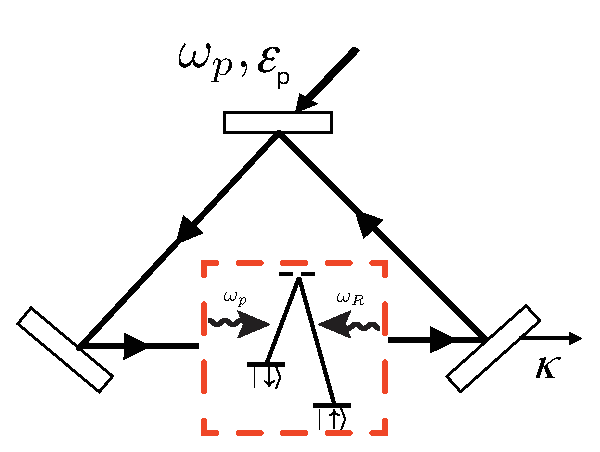
\includegraphics[width=0.65\textwidth]{schematic}\caption{Schematic diagram of the cavity-assisted spin-orbit coupled system. Inside the red dashed box, we show the level diagram of the atom and the light field configuration where $\omega_p$ represents the cavity field and $\omega_R$ is an external coherent laser beam. $\epsilon_p$ and $\kappa$ are the cavity pumping rate and decay rate, respectively.}\label{schematic}
\end{figure}

\section{Model Setup and Mean-Field Formalism} \label{meanfield}

As shown schematically in Fig.~\ref{schematic}, we consider a single atom being confined by a single-mode unidirectional ring cavity, whose cavity mode together with an additional coherent laser beam form a pair of Raman beams that induces transition between two hyperfine atomic ground states denoted as $|\uparrow\rangle$ and $|\downarrow\rangle$, while transferring recoil momentum $\pm 2\hbar q_r\hat{z}$ to the atom. The ring cavity has a resonant frequency of $\omega_c$, decay rate $\kappa$, and is pumped by an external laser field with frequency $\omega_p$ and pumping rate $\varepsilon_p$.
The Hamiltonian under the rotating wave approximation can be written as \cite{cavitySOC},
\ba
 \mathcal{H}_{\rm eff}& = & \sum_{\sigma=\uparrow,\downarrow} \int d{z}\left[ \hat{\psi}^\dagger_\sigma({z})\left(\frac{ { k}^2+ 2\alpha_\sigma q_r {k}}{2m}+\alpha_\sigma \delta\right)\hat{\psi}_\sigma(z)\right]+  \frac{\Omega}{2}\int d{z}\left[\hat{\psi}_{\uparrow}^{\dagger}({z})\hat{\psi}_{\downarrow}({z}) \hat{c}+ h.c. \right]\nonumber \\
 & + & i\varepsilon_{p}(\hat{c}^{\dagger}-\hat{c})-\delta_c \hat{c}^{\dagger}\hat{c} \,, \label{effH}
 \ea
where, for simplicity, we only consider the atomic COM motion along the $z$-axis, which is the direction of the photon recoil. In Hamiltonian (\ref{effH}), $k$ is the atomic COM quasi-momentum (we take $\hbar =1$) along the $z$-axis, $\hat{c}$ is the cavity annihilation operator, $\hat{\psi}_\sigma(z)$ ($\sigma = \uparrow$, $\downarrow$) is the atomic operator, $\alpha_{\uparrow, \downarrow}=\pm 1$, $2\delta$ represents the two-photon Raman detuning, $\delta_c=\omega_p-\omega_c$ is the cavity-pump detuning, and $\Omega$ denotes the atom-cavity coupling strength (or more specifically, the Raman coupling strength per cavity photon). Finally we will treat the cavity decay phenomenologically, which amounts to adding a non-Hermitian term $-i\kappa \hat{c}^{\dagger}\hat{c}$ in the above effective Hamiltonian. Note that for a quasi-momentum $k$, the real momentum for an atom is spin-dependent: it is $k+q_r$ for $|\uparrow \rangle$ state and $k-q_r$ for $|\downarrow \rangle$ state.

From Hamiltonian~(\ref{effH}), one can easily obtain the Heisenberg equations of motion for both atomic and cavity fields. To proceed, we adopt the mean-field approximation by replacing the operators by their respective expectation values: $\hat{c} \rightarrow c\equiv \langle \hat{c} \rangle \,, \hat{\psi}_\sigma ({z}) \rightarrow  \psi_\sigma (z)\equiv \langle \hat{\psi}_\sigma ({z}) \rangle $.
%The mean-field approximation is justified by assuming small quantum fluctuations of both operators $c$ and $\psi_\sigma({\bf r})$.
Assuming spatial homogeneity, we further take the plane-wave wave-function for the atomic modes $\psi_\sigma({z})=e^{i{k} {z}}\varphi_\sigma$ with the normalization condition $|\varphi_\uparrow|^2+|\varphi_\downarrow|^2=N_{\rm atom}$, where $N_{\rm atom}$ is the total number of atoms which we take to be 1 in the current work. The steady-state solution for the photon field is obtained by taking the time derivative of the photon field to be zero, from which we obtain:
\begin{equation}
c = \frac{\varepsilon_{p}-i\frac{\Omega}{2} \varphi_\downarrow^\ast\varphi_\uparrow}{\kappa-i\delta_{c}}.
\label{c}
\end{equation}
Inserting this into the equations for atomic fields, we obtain the coupled nonlinear time-dependent equations for the two spin components as,
\ba
i\dot{\varphi}_{\uparrow}&\!\! =\!\! & \left(\frac{{k}^{2}}{2m}+q_{r}k+\delta\right) \varphi_{\uparrow}+ \frac{\Omega_{\rm eff}}{2}\, \varphi_{\downarrow} \,,\label{EOMphi1}\\
i\dot{\varphi}_{\downarrow} & \!\!= \!\!& \left(\frac{{k}^{2}}{2m}-q_{r}k-\delta\right)\varphi_{\downarrow}+ \frac{\Omega^*_{\rm eff}}{2}\,\varphi_{\uparrow}\,.\label{EOMphi2}
\ea
where $\Omega_\text{eff} \equiv {\Omega} c ={\Omega} \frac{\varepsilon_{p}-i\frac{\Omega}{2} \varphi_\downarrow^\ast\varphi_\uparrow}{\kappa-i\delta_{c}} $ is the effective Raman coupling strength between two atomic states. The fact that $\Omega_{\rm eff}$ depends on the atomic field itself is a manifestation of the non-linearity arising from the atomic back-action to the cavity field.

For a given atomic quasi-momentum ${k}$, we define eigenstate and eigenenergy as the solution of the time-independent version of Eqs.~(\ref{EOMphi1}) and (\ref{EOMphi2}), by replacing $i(\partial/\partial t)$ with $\epsilon({k})$. After some lengthy but straightforward algebra, we find that $\epsilon({ k})$ obeys a quartic equation in the form of
% (we consider $\mathcal{N}=1$ hereafter):
\begin{equation}
4\epsilon^4+B\epsilon^3+C\epsilon^2+D\epsilon+E=0 \,.
\label{generalquarticEq}
\end{equation}
The derivation of the above equation and the explicit expressions of the $k$-dependent coefficients $B$, $C$, $D$ and $E$ can be found in our previous work \cite{cavitySOC}.

\begin{figure}[htp]
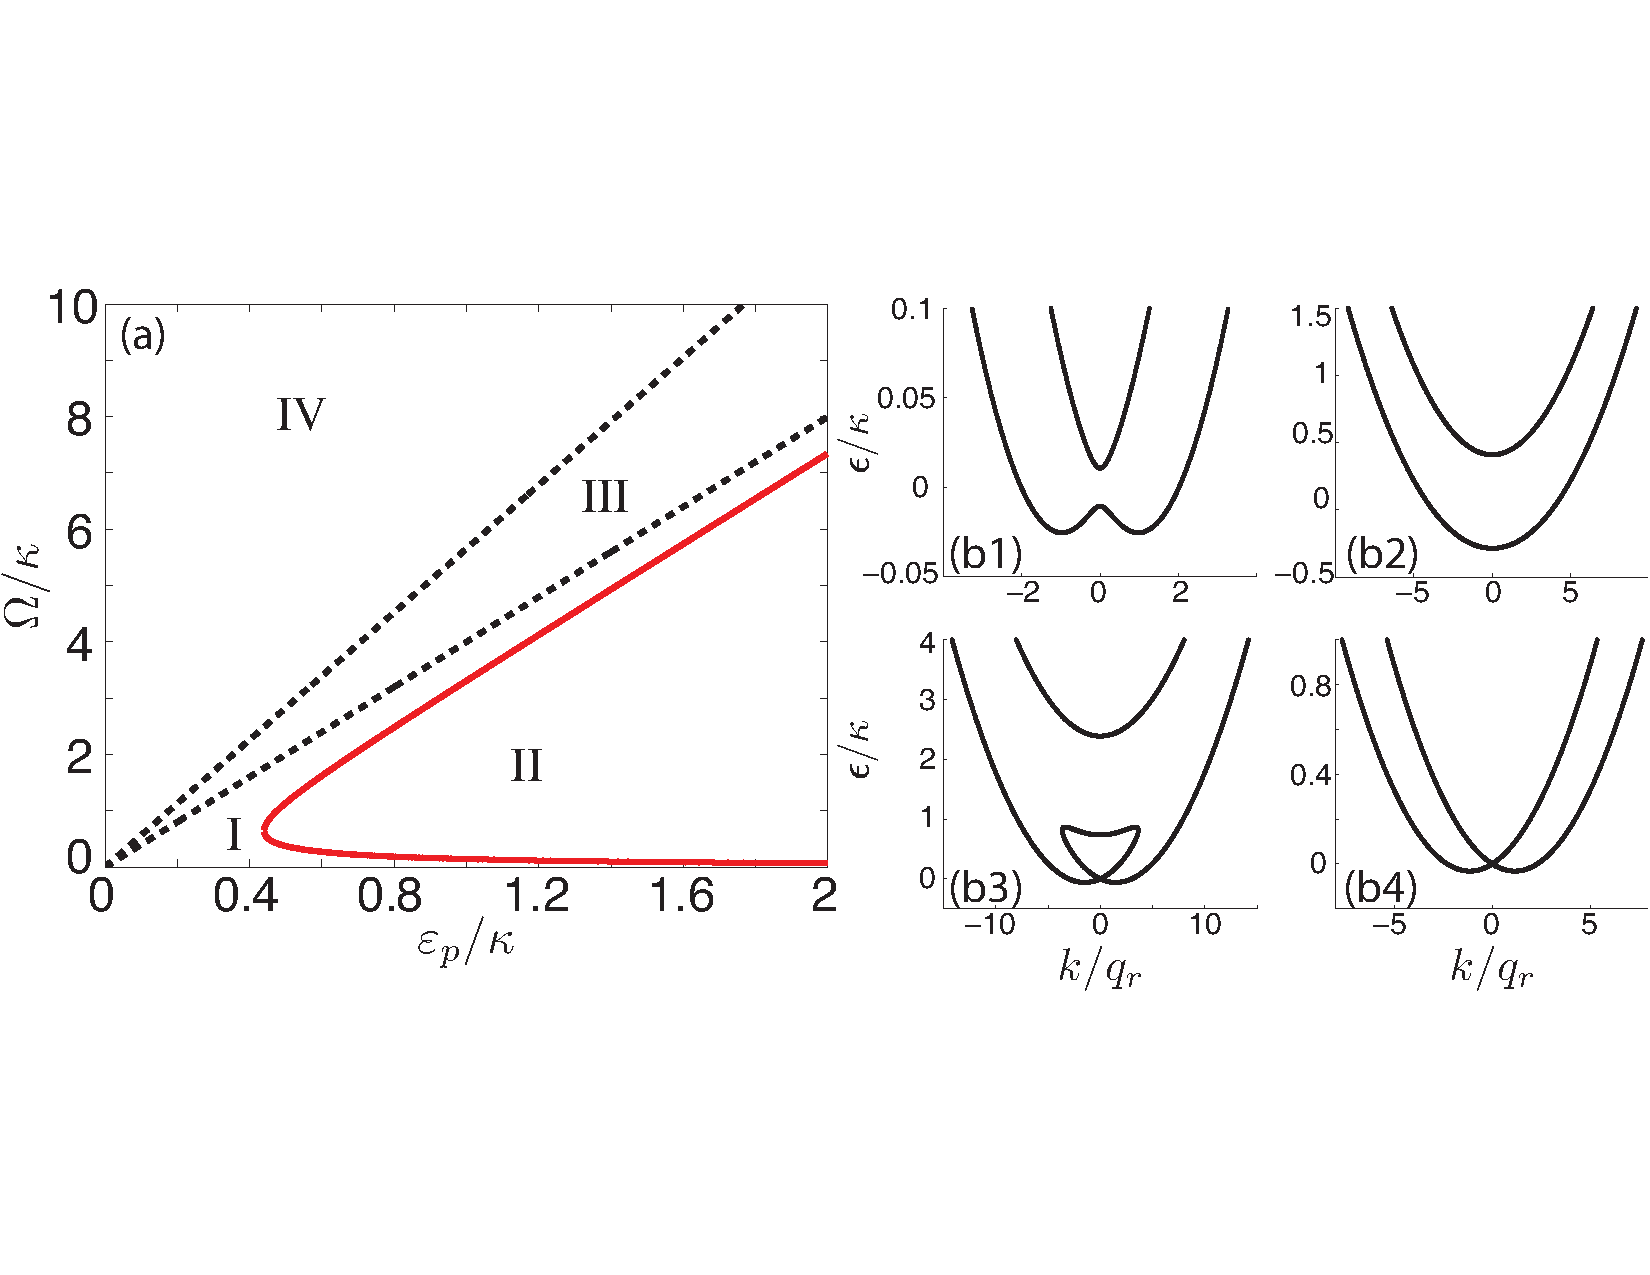
\includegraphics[width=0.95\textwidth]{fig1}\caption{Single particle eigen-energy spectrum ``phase diagram''.  The dispersion curve is generally catagorized by four regions, represented from I to IV in (a). From (b1) to (b4), we fix $\varepsilon_p=\kappa$. In region I, the dispersion has double minima as shown in (b1) with $\Omega=0.03\kappa$; region II is enclosed by the red solid curve in (a) and we show the typical point in (b2) ($\Omega=\kappa$) where only single minimum exisits in the lower helicity branch; region III is enclosed by the black dashed lines in (a) and it is a region where loop structure emerges, as in (b3) with $\Omega=5\kappa$; finally, in region IV we recover the double minimum dispersion although it's different from region I by closing the gap at $k=0$, as in (b4) with $\Omega=8\kappa$. Throughout the paper we fix $\delta_c=\kappa$ and $\delta=0$, and adopt a dimensionless unit system with $\hbar=m=\kappa=1$. A typical value for $\kappa$ is $2\pi \times 1 \text{ MHz}$, and we choose $q_r = 0.22$ in our dimensionless units (based on a realistic experimental parameter estimate). }\label{fig1}
\end{figure}

We can gain some insights about the general structure of the dispersion relation $\epsilon(k)$, e.g. the degeneracy condition and the appearance and disappearance of the loop. In the case of vanishing two-photon detuning (i.e., $\delta=0$),
simple analysis shows that there should be a total of four regimes, as shown in Fig.~\ref{fig1}(a). In region I, the two dispersion branches are gapped, and the lower branch has a double degenerate minima, as shown in Fig.~\ref{fig1}(b1). This dispersion curve structure is very similar to the case when both Raman beams are provided by classical coherent laser fields (we shall refer to this as the ``classical case'') and the Raman coupling strength is small. In region II, as shown in Fig.~\ref{fig1}(b2), the two dispersion branches are still gapped, but the lower branch has a single minimum. This is similar to the classical case with a large Raman coupling strength. Regions III and IV do not have analogs in the classical case. Region III features a loop structure, as shown in Fig.~\ref{fig1}(b3), whereas in Region IV, the loop dissolves but the two dispersion branches becomes gapless at $k=0$, as shown in Fig.~\ref{fig1}(b4). In the looped region, the quartic equation (\ref{generalquarticEq}) yields four real roots. It can be shown \cite{cavitySOC} that this requires the coupling strength $\Omega$ to satisfy
\[\Omega_c^{(1)}\equiv4\varepsilon_p\leq \Omega \leq  4\varepsilon_p \sqrt{1+(\delta_c/\kappa)^2}\equiv\Omega_c^{(2)} \,.\]
The two dashed lines in Fig.~\ref{fig1}(a) represent the two critical values $\Omega_c^{(1)}$ and $\Omega_c^{(2)}$, respectively.

\begin{figure}[htp]
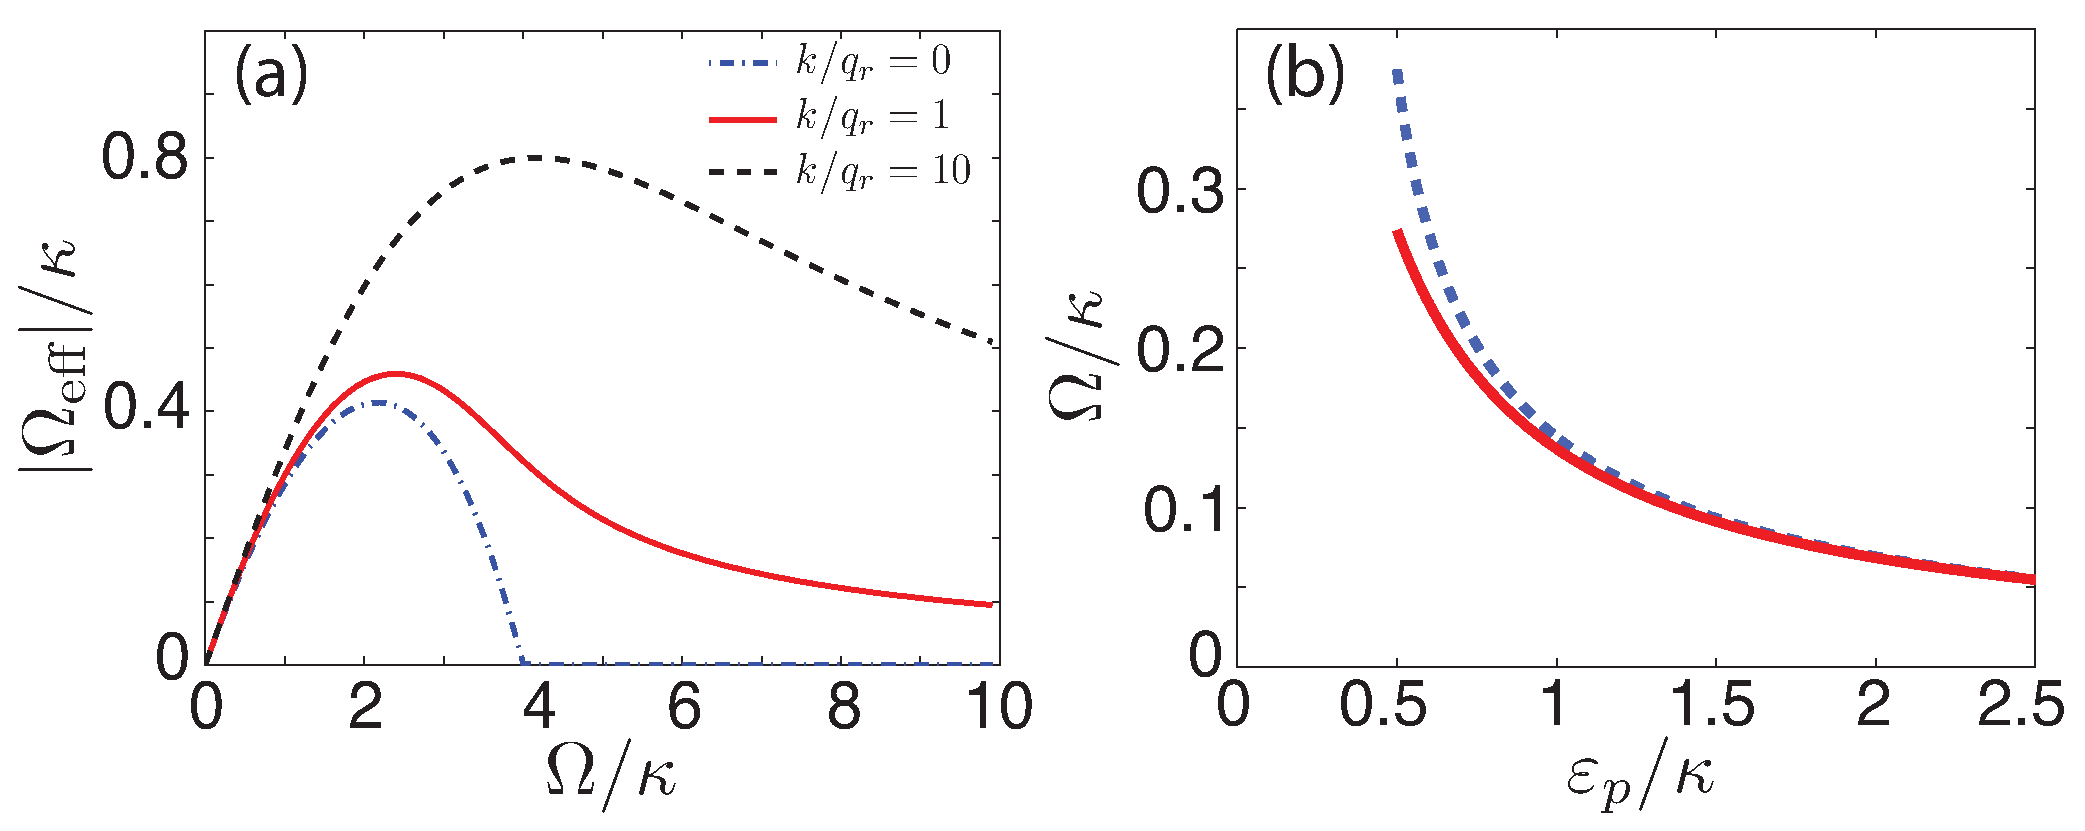
\includegraphics[width=0.95\textwidth]{fig2}\caption{(a) Effective Raman coupling $|\Omega_\text{eff}|$ is plotted as a function of atom-photon coupling strength $\Omega$ for different $k$ values, $0$,\,$q_r$,\,$10q_r$ for blue dash-dot, red solid and black dashed  lines. We observe that $|\Omega_\text{eff}|$ does not monotonically  increases with $\Omega$ but rather peaks at an intermediate value, then approaches zero in the large $\Omega$ limit. Figure (b) shows a comparison between critical boundary of region I and II (red solid curve) and the analytical result (blue dashed line) given in Eq.~(\ref{ome}). At large $\varepsilon_p$ limit, the two results match asymptotically well.  }\label{fig2}
\end{figure}

It is instructive to examine how the effective Raman coupling strength $\Omega_{\rm eff}$ behaves as a function of $\Omega$. In Fig.~\ref{fig2}(a), we plot $|\Omega_\text{eff}|$ for the lowest dispersion branch as a function of $\Omega$ for different $k$ values. Note that $|\Omega_{\rm eff}|^2 = \Omega^2 n_{\rm photon}$ where $n_{\rm photon}=|c|^2$ is the steady-state cavity photon number. A few remarks can be made based on this plot. First, the fact that $\Omega_{\rm eff}$ is different for different $k$ clearly shows the influence of the atomic COM motion on both the atomic internal dynamics and the cavity photon number. Second, $|\Omega_{\rm eff}|$ is not a monotonous function of $\Omega$. For given $k$, $|\Omega_{\rm eff}|$ increases with $\Omega$ linearly for small $\Omega$. This can be intuitively understood as follows. At such weak atom-photon coupling, the back-action from the atom to the cavity photon is negligible. The number of cavity photons $n_{\rm photon}$ is roughly given by $n_{\rm photon} \approx n_0=\left|\frac{\varepsilon_{p}}{\kappa-i\delta_{c}}\right|^2= \frac{\varepsilon_p^2}{\kappa^2+ \delta_c^2}$, where $n_0$ is the number of cavity photons when the atom is absent. As a result, we have $|\Omega_{\rm eff}| \approx \Omega \sqrt{n_0}$ which is independent of the atomic quasi-momentum $k$. On the other limit, when $\Omega$ is very large, the strong atom-cavity coupling strength significantly detunes the cavity away from resonance and the cavity photon number $n_{\rm photon}$, and hence $|\Omega_{\rm eff}|$, decreases as a function of $\Omega$. Such a non-monotonous behavior of $\Omega_{\rm eff}$ is a unique feature of the cavity system and a direct manifestation of the non-linearity of the system arising from the back-action of the atom on the cavity photon.

From the above analysis, it should also become clear that when the effect of the back-action is weak (which occurs when $\Omega$ is small and/or $\varepsilon_p$ is large), we should recover the properties of the classical case. In particular, in the classical case, the lower dispersion branch change from two degenerate minima to a single minimum when the Raman coupling strength exceeds a critical value. Using our notation, this occurs when $|\Omega_{\rm eff}|$ exceeds the critical value $4E_r$ where $E_r=q_r^2/(2m)$ is the photon recoil energy. For weak atom-cavity coupling, $|\Omega_{\rm eff}| = \Omega \sqrt{n_0}={\Omega} \frac{\varepsilon_p}{\sqrt{\kappa^2+ \delta_c^2}}$. Hence the critical value of $\Omega$ is given by
\begin{equation}
\Omega=4E_r\frac{\sqrt{\kappa^2+\delta_c^2}}{\varepsilon_p}\,.
\label{ome}
\end{equation}
In Fig.~\ref{fig2}(b), we plot this critical value (blue dashed line) as a function of cavity pump rate $\varepsilon_p$ and compare it with the numerically determined lower boundary (red solid line) between region I and II of Fig.~\ref{fig1}(a). The two curves overlap with each other when $\varepsilon_p$ increases. Therefore, as we have expected, in the limit of weak atom-cavity coupling and strong cavity pumping, we fully recover the classical case where the SOC is induced by two classical laser beams.


\section{Master Equation Approach: Full Quantum Mechanical Treatment } \label{master}

The above discussion is based on the mean-field approach where the cavity field is replaced by a $c$-number that represents the photon amplitude. This mean-field treatment relies on two implicit assumptions: (1) the atom-photon correlation is negligible, and (2) the photon field can be well approximated by a coherent state. In order to examine the validity of these assumption, and hence the validity of the mean-field approximation, we now turn to a full quantum treatment based on the Master equation:
\be
\dot{\rho} = \frac{1}{i\hbar}[{\cal H}_{\text{eff}},\rho]+\mathcal{L}[\rho] \,. \label{masterEq}
\ee
Here $\rho$ is the total density operator of the coupled atom-cavity system, the effective Hamiltonian ${\cal H}_{\text{eff}}$ is the same as in Eq.~(\ref{effH}). The dissipation arising from cavity decay is modeled by the Liouvillean term in the
standard form of Lindblad super-operator \cite{L1, L2},
\be
\mathcal{L}[\rho] = \kappa (2c\rho \hat{c}^\dagger-\hat{c}^\dagger \hat{c}\rho-\rho \hat{c}^\dagger \hat{c})\,.\label{Lindblad}
\ee
Again, due to spatial homogeneity, we decouple momentum eigenstates by taking the plane-wave ansatz for the atomic modes as $\hat{\psi}_\sigma({z})=e^{i{k}{z}}\hat{\psi}_\sigma$. As there is no coupling between atomic operators with different $k$, we can work in the subspace for a fixed value of $k$. Here we explicitly write the commutator in Eq.~(\ref{masterEq}), for a given atomic quasi-momentum $k$, as,
\ba
[{\cal H}_{\text{eff}}({k}),\rho] & = & \left(\frac{{ k}^{2}}{2m}+\frac{q_{r}k}{m}+\delta\right)\left(\hat{\psi}_{\uparrow}^{\dagger} \hat{\psi}_{\uparrow}\rho-\rho \hat{\psi}_{\uparrow}^{\dagger} \hat{\psi}_{\uparrow}\right)+\left(\frac{{k}^{2}}{2m}-\frac{q_{r}k}{m}-\delta\right) \left(\hat{\psi}_{\downarrow}^{\dagger} \hat{\psi}_{\downarrow}\rho-\rho \hat{\psi}_{\downarrow}^{\dagger} \hat{\psi}_{\downarrow}\right)\nonumber\\
 &  & + \frac{\Omega}{2}\left(\hat{\psi}_{\uparrow}^{\dagger} \hat{\psi}_{\downarrow} \hat{c} \rho+\hat{c}^{\dagger} \hat{\psi}_{\downarrow}^{\dagger} \hat{\psi}_{\uparrow}\rho-\rho \hat{\psi}_{\uparrow}^{\dagger} \hat{\psi}_{\downarrow}c-\rho \hat{c}^{\dagger} \hat{\psi}_{\downarrow}^{\dagger} \hat{\psi}_{\uparrow}\right)\nonumber\\
&& + i\varepsilon_{p}\left(\hat{c}^{\dagger}\rho-\hat{c}\rho-\rho \hat{c}^{\dagger}+\rho \hat{c}\right)-\delta_{c}\left(\hat{c}^{\dagger}\hat{c}\rho-\rho \hat{c}^{\dagger}\hat{c}\right)\,.
\ea
Note that if the photon recoil $q_r=0$, which occurs when the cavity mode and the external laser beams are co-propagating, the COM kinetic energy terms $k^2/(2m)$ can be gauged away after a simple gauge transformation. Our model is then reduced to the J-C model and the atomic COM motion does not play a role.
To solve the Master equation (\ref{masterEq}), we choose our basis states as direct product states of photon Fock state $|n \rangle$ and atomic internal state $|\sigma=\uparrow,\downarrow \rangle$: $|n;\sigma\rangle \equiv |n \rangle \otimes |\sigma \rangle$, %$n=0,1,2,...,\infty$
where non-negative integer $n$ denotes cavity photon number. Our goal is to calculate the entire matrix elements of the density operator under this set of basis states, denoted by $\langle m;\sigma|\rho|n;\sigma'\rangle\equiv\rho_{mn}^{\sigma\sigma'}$. We found the governing equation for the matrix element can be written as,
\ba
\frac{d}{dt}\rho_{mn}^{\sigma\sigma'}
& = & -i\left(\frac{{k}^{2}}{2m}+\frac{q_{r}k}{m}+ \delta\right)\left(\delta_{\sigma\uparrow}-\delta_{\sigma'\uparrow}\right)\rho_{mn}^{\sigma\sigma'}
-  i\left(\frac{{k}^{2}}{2m}-\frac{q_{r}k}{m}-\delta\right)\left(\delta_{\sigma\downarrow}-\delta_{\sigma'\downarrow}\right)\rho_{mn}^{\sigma\sigma'}\nonumber\\
& + & \frac{\Omega}{2i}(\delta_{\sigma\uparrow}\sqrt{m+1}\rho_{m+1n}^{\bar{\sigma}\sigma'}
+\delta_{\sigma\downarrow}\sqrt{m}\rho_{m-1n}^{\bar{\sigma}\sigma'}
-\delta_{\sigma'\uparrow}\sqrt{n+1}\rho_{mn+1}^{\sigma\bar{\sigma'}}
-\delta_{\sigma'\downarrow}\sqrt{n}\rho_{mn-1}^{\sigma\bar{\sigma'}})\nonumber\\
& + & \varepsilon_{p}\left(\sqrt{m}\rho_{m-1n}^{\sigma\sigma'}-\sqrt{m+1}\rho_{m+1n}^{\sigma\sigma'}+\sqrt{n}\rho_{mn-1}^{\sigma\sigma'}-\sqrt{n+1}\rho_{mn+1}^{\sigma\sigma'}\right)\nonumber\\
& + & i\delta_{c}\left(m-n\right)\rho_{mn}^{\sigma\sigma'}
+ \kappa\left(2\sqrt{m+1}\sqrt{n+1}\rho_{m+1n+1}^{\sigma\sigma'}-(m+n)\rho_{mn}^{\sigma\sigma'}\right),\label{EOMrho}
\ea
where $\bar{\sigma}$ represents the flip-spin value, i.e. $\bar{\uparrow}=\downarrow$ and $\bar{\downarrow}=\uparrow$.

With Eq.~(\ref{EOMrho}), we can study the dynamical evolution of the density operator $\rho$ for a given initial state. Obviously, we need to introduce a sufficiently large photon number cutoff. Once we obtain the density operator, all relevant physical quantities can be readily calculated. An example is given in Fig.~\ref{evo}, where we show the time evolution of the cavity photon number $n = {\rm Tr}[\rho \hat{n}]= {\rm Tr}[\rho \hat{c}^\dag \hat{c}]$ for the initial state $|0; \uparrow \rangle$. The three different curves in Fig.~\ref{evo} correspond to different atomic quasi-momentum $k$.

\begin{figure}[htp]
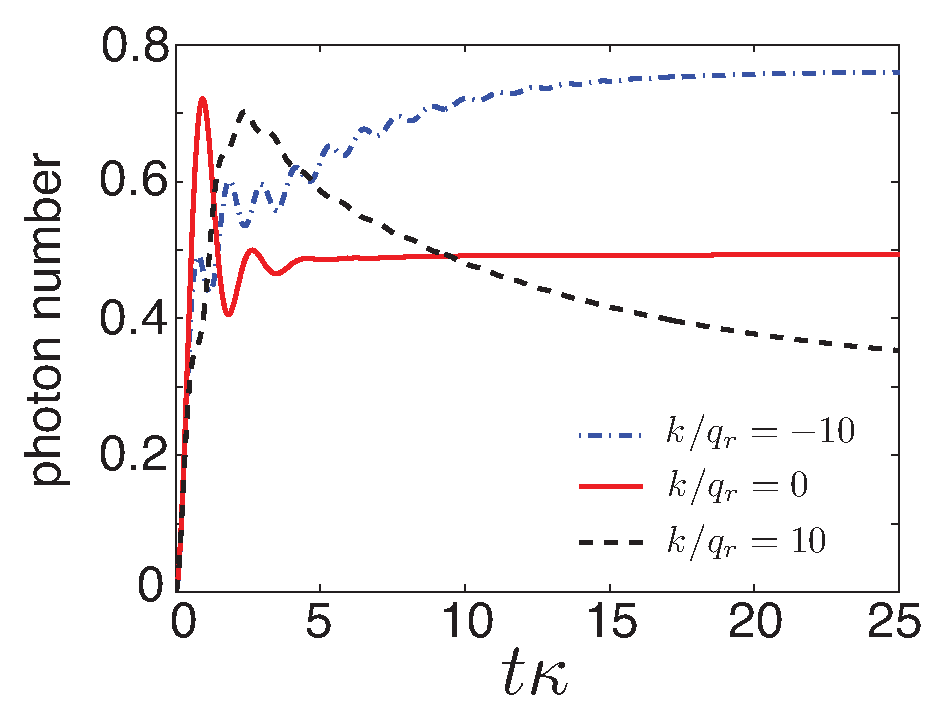
\includegraphics[width=0.65\textwidth]{photon_evolution}\caption{Time evolution of cavity photon number. The initial state is given by $|0;\uparrow\rangle$ and we consider the same parameter as in Fig.~\ref{photon}(a) with $k/q_r=-10,\,0,\,10$. The steady-state values, obtained in the long time limit as shown here, correspond to red dashed lines at corresponding $k$ values in Fig.~\ref{photon}(a).}\label{evo}
\end{figure}

As evidenced in Fig.~\ref{evo}, due to the presence of cavity decay, a steady state will eventually be reached. Let us now focus on the properties of the steady state. The steady-state density operator matrix elements can be obtained by equating the RHS of Eq.~(\ref{EOMrho}) to zero. The red dashed lines in Fig.~\ref{photon}(a)-(c) represent the steady-state photon number as functions of atomic quasi-momentum $k$. The horizontal arrows in the plot represent the cavity photon number by setting $q_r=0$, in which case our model reduces to the J-C model and all physical quantities become $k$-independent.

To have a better understanding of the photon statistics, we study the steady-state photon number fluctuation. Specifically, we calculate the normalized photon number fluctuation defined as
\[\Delta_n = \frac{\langle(\Delta n)^{2}\rangle}{\langle \hat{n}\rangle}=\frac{\langle \hat{n}^{2}\rangle-\langle \hat{n}\rangle^{2}}{\langle n\rangle} \,,\]
where the expectation values of the operators are obtained with the help of the steady-state density operator. For a coherent cavity field, the photon fluctuation is Poissonian and we have $\Delta_n=1$.
The solid curves in Fig.~\ref{photon}(d)-(f) represent $\Delta_n$ (left vertical axis) as functions of $k$, and the horizontal arrows pointing to left give the values of $\Delta_n$ from the J-C model by setting $q_r=0$. For the parameters we have used, we note that the J-C model always predicts a super-Poissonian photon statistics, whereas our model gives super-Poissonian photon statistics only for small atomic quasi-momentum, but Poissonian statistics as $k/q_r \rightarrow \pm \infty$.

Last but not least, to characterize the correlation between the atom and the cavity field, we investigate the so-called negativity \cite{negativity} which measures the degree of entanglement for a mixed state system.
The negativity is defined as $\mathcal{N}(\rho)=(||\rho^{T_A}||_1-1)/2$, where $\rho^{T_A}$ is the partial transpose of the density operator with respect to either the atom subsystem or the cavity subsystem, and $||\rho^{T_A}||_1$ denotes its trace norm with the definition $||\hat{A}||_1 \equiv {\rm Tr}[\sqrt{\hat{A}^\dag \hat{A}} ]$. A negativity of zero indicates that the two subsystems (the atom and the cavity, in our case) are not entangled, whereas a positive negativity means that finite degree of entanglement is present. The dashed curves in Fig.~\ref{photon}(d)-(f) represent the negativity (right vertical axis) in the steady state as functions of $k$, and the horizontal arrows pointing to right give the values of the negativity from the J-C model by setting $q_r=0$. One can observe that for the chosen parameters, the J-C model always predicts a finite degree of entanglement between the atom and the cavity field. By contrast, the degree of entanglement in our model weakens when $k/q_r \rightarrow \pm \infty$.

\begin{figure}[htp]
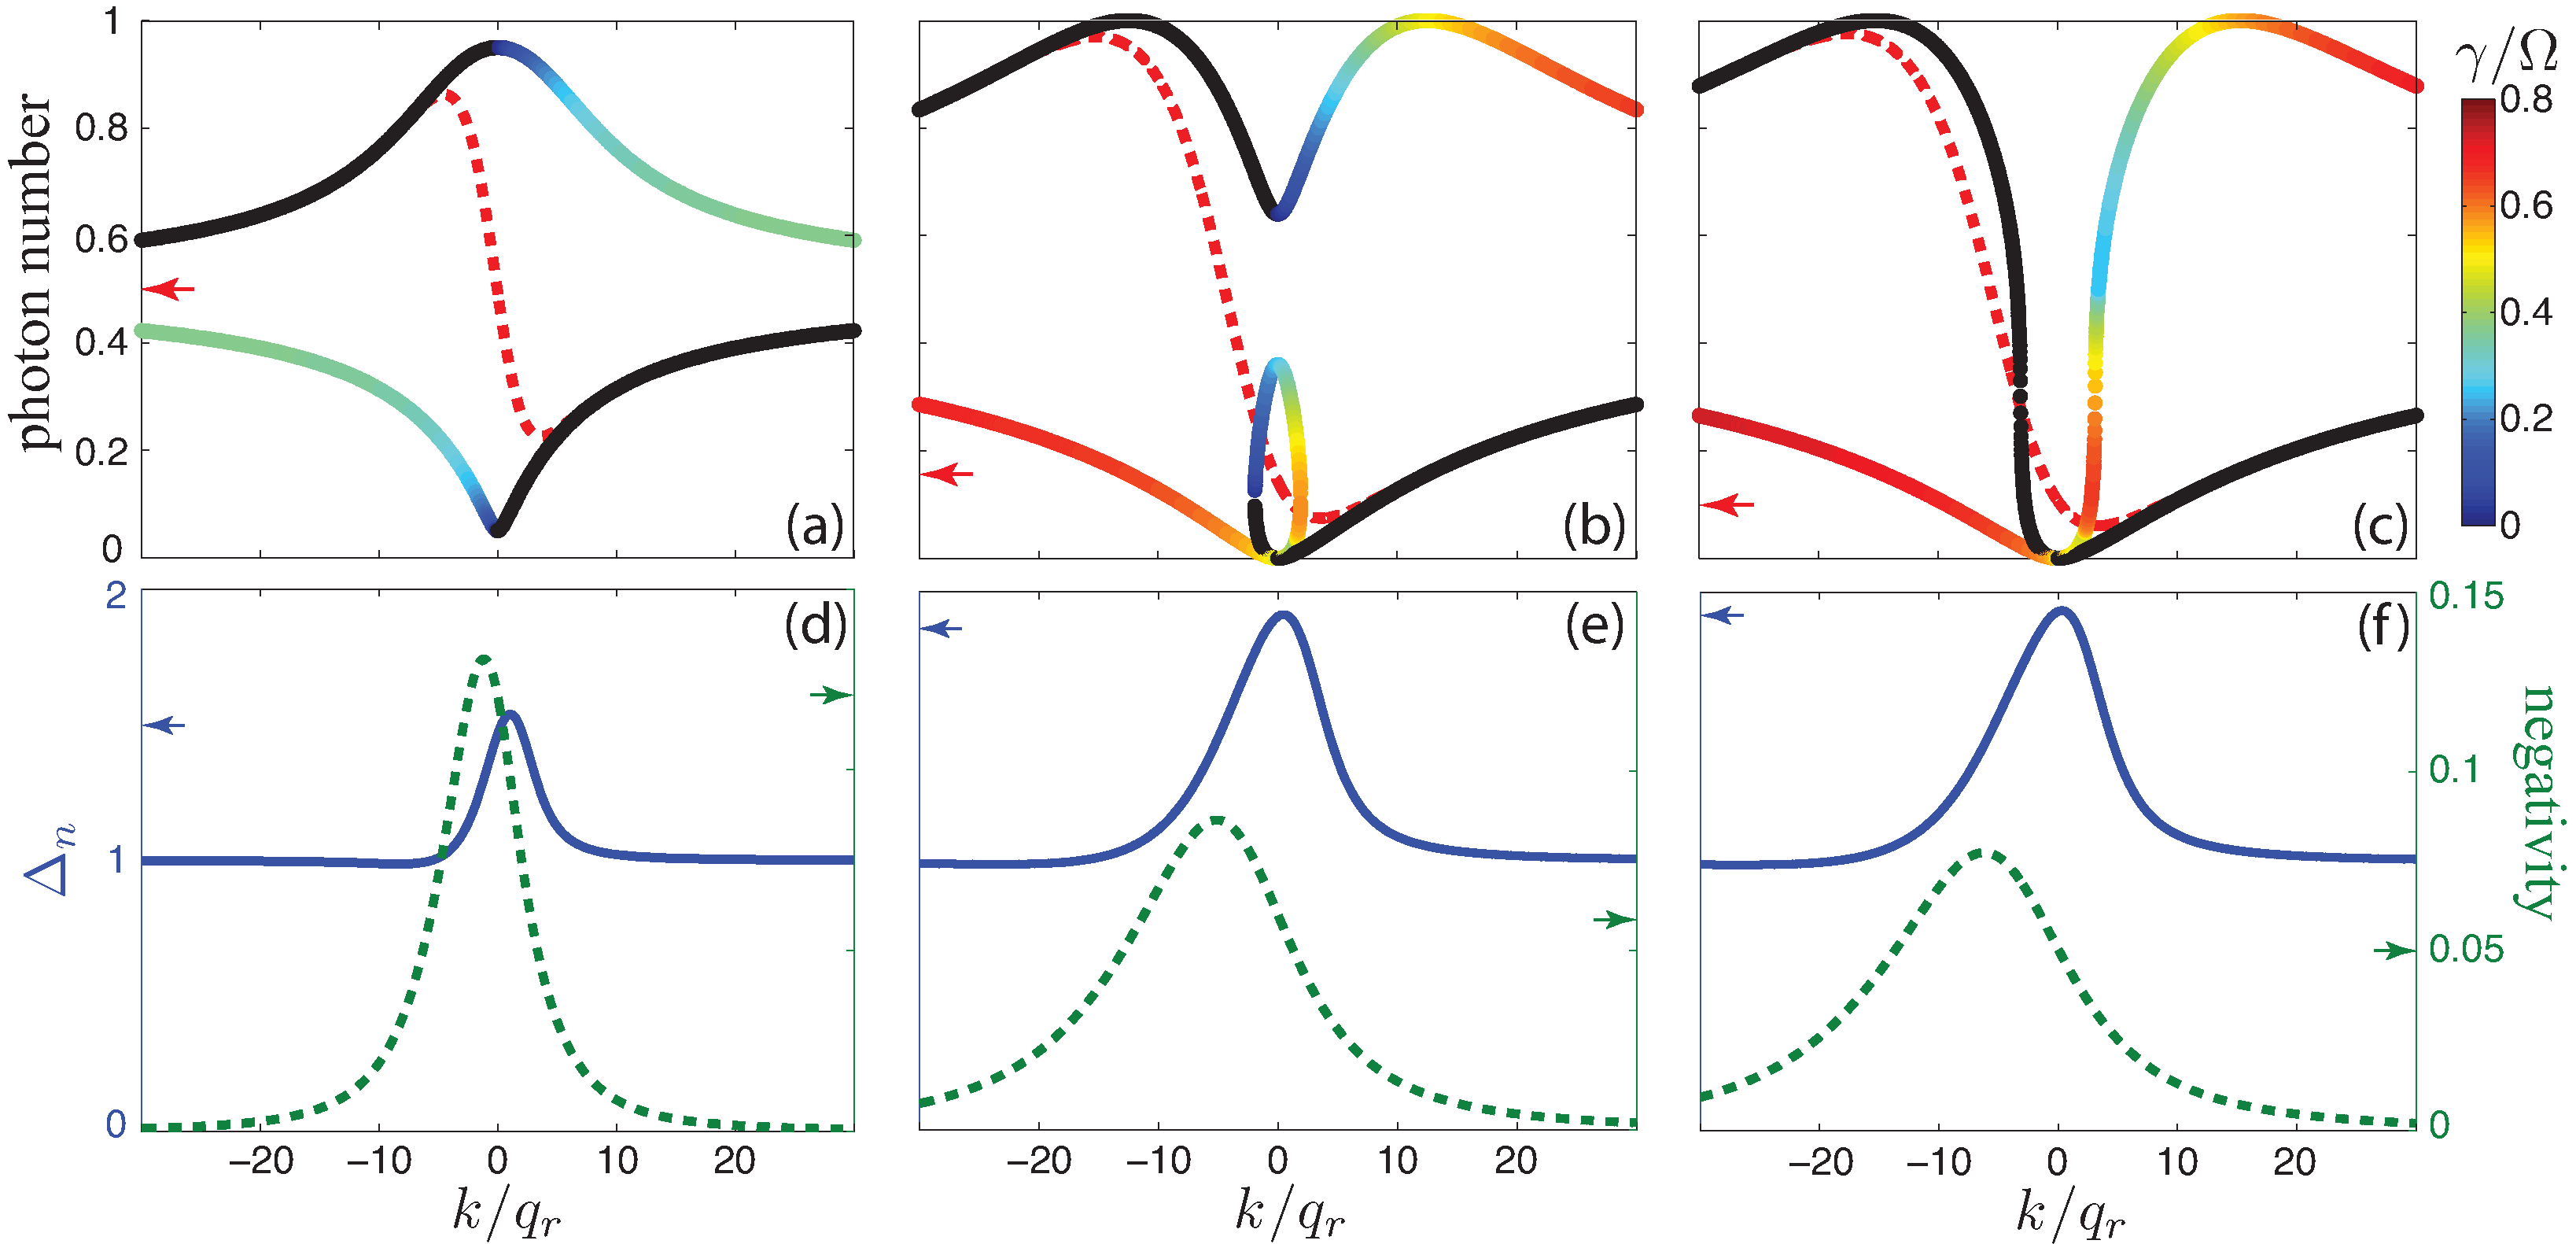
\includegraphics[width=0.95\textwidth]{photon}
\caption{(a)$\sim$(c) Photon number obtained from the mean-field approach (solid curves) and from quantum mechanical Master equation approach (red dashed curves). From (a) to (c), $\Omega = 3\kappa,\ 5.6\kappa,\ 6\kappa$. The color on the solid curves represents the normalized decay rate $\gamma/\Omega$ of unstable mean-field states. The black color represents stable mean-field states. We have used $\varepsilon_p=\kappa$, and other parameters are the same as in Fig.~\ref{fig1}. (d)$\sim$(f) Corresponding photon number fluctuation (blue solid curve) and negativity (green dashed line) obtained from the quantum approach. The parameters used here are the same in (a)$\sim$(c), respectively. The horizontal arrows indicate results from the J-C model by taking $q_r=0$.
%At the large $k_z$ limit, we found $\text{Tr}[\rho_\text{photon}n]$ asymtotes to semi-classical mean field result $|\langle c\rangle|^2$, which further matches stable branches according to mean field stability analysis.
}\label{photon}
\end{figure}

\section{Discussions} \label{relation}

In the previous two sections, we have presented two different methods for studying the system. We are now in a position to discuss their connections.

In Fig.~\ref{photon}(a)-(c), in addition to the steady-state photon number obtained from the quantum treatment (dashed curves), we also plot the photon number $n_{\rm photon}=|c|^2$ obtained from the mean-field approach (solid curves), with $c$ given in Eq.~(\ref{c}). In the quantum treatment, the steady-state density matrix is obtained by solving a set of linear equations. For a given $k$, the solution is unique. Hence we only get one steady-state photon number for a given atomic quasi-momentum. On the other hand, the mean-field treatment allows multiple steady-state solutions corresponding to different real roots of the quartic equation Eq.~(\ref{generalquarticEq}). Hence a single $k$ value is associated with more than one steady-state photon number. However, due to the non-linearity intrinsic in the mean-field method, not all steady-states are dynamically stable. A straightforward stability analysis allows us to quantify the dynamical stability of the mean-field states, as we did in Ref.~\cite{cavitySOC}. The stability information of the mean-field states are encoded as the color value in the solid curves. Those stable states are represented by black color, while any color other than black indicates an unstable state, and the color value represents the decay rate (see the colorbar) of the corresponding state. From Fig.~\ref{photon}(a)-(c), we clearly see that at large atomic quasi-momentum $k/q_r \rightarrow  \pm \infty$, the Master equation result overlaps with the stable mean-field branch; while at small $|k|$, the quantum result deviates significantly away from the mean-field solution.

The agreement for large $|k|$ and the discrepancy at small $|k|$ are both consistent with the results of the negativity and photon number fluctuations as presented in Fig.~\ref{photon}(d)-(f): At large $|k|$, the negativity is small (i.e., atom-cavity entanglement is weak) and the photon number fluctuation tends to Poissonian (i.e., the photon field is well approximated by a coherent state), this is exactly the regime where we expect the mean-field approximation is valid. By contrast, for small $|k|$, the quantum calculation indicates that there is non-negligible entanglement between the atom and the cavity field, and the cavity field itself cannot be assumed as a coherent state. Hence the mean-field assumption is no longer valid.

The reason why mean-field approximation only works for large $|k|$ is actually rather simple. Consider a Raman transition process where the atom jumps from $|\uparrow \rangle$ to $|\downarrow \rangle$. The quasi-momentum $k$ does not change during this process, however the real momentum changes from $k+q_r$ to $k-q_r$. Therefore the effective two-photon Raman detuning is not just $2\delta$, but $2\delta +2q_rk/m$, where the additional term comes from the difference of the kinetic energies for different pseudo-spin state $|\sigma\rangle$. In other words, the SOC renders the two-photon detuning momentum-dependent. In the examples we presented in this work, we have taken $\delta=0$. Hence the Raman transition is only near-resonant for small $|k|$, and becomes far off-resonant for large $|k|$. Therefore, for large $|k|$, the atom-photon coupling, and hence the atomic back-action to cavity, are weak. This explains why the mean-field assumption becomes valid in this regime.


\section{Conclusion} \label{conclusion}

In this work, we have studied spin-orbit coupled cold atoms inside a ring cavity system, employing both the mean-field theory and the full quantum mechanical Master equation approach. By treating both light and atom on equal footing and seeking the self-consistent solution in both approaches, we have found: (1) cavity-assisted SOC dramatically modifies atomic dispersion relation, (2) intriguing dynamical instabilities exist in the system, (3) atom's back-action onto cavity field also leads to non-trivial atom-photon coupling that is fundamentally different from either the system with classical-laser induced SOC in the absence of the cavity or the J-C model where the atomic COM motion is neglected (i.e., by taking $q_r=0$). We have also explored correspondence and discussed the connection between the mean-field and the quantum approaches. The two distinctively different approaches provide us with a deeper understanding and complementary insights into this system. We conclude that the synthesis of cavity QED and SOC is not a trivial combination and interesting new physics emerges in this setting.



\acknowledgments{Acknowledgments}
This work is supported by the US National Science Foundation and the Welch Foundation (Grant No. C-1669);
\authorcontributions{Author Contributions}
H.P. conceived the idea of the project, L.D. and C. Z. explored the theoretical and numerical aspects of the physics. All authors contributed to writing and revising the manuscript and participated in the discussions about this work.
\conflictofinterests{Conflicts of Interest}
The authors declare no conflict of interest.

%=================================================================
% References: Variant A
%=================================================================
% Back Matter (References and Notes)
%----------------------------------------------------------
% Style and layout of the references
% Reference 1
% \bibitem{ref-journal}
% Lastname, F.; Author, T. The title of the cited article. {\em Journal Abbreviation} {\bf 2008}, {\em 10}, 142-149
\bibliographystyle{mdpi}
\makeatletter
\renewcommand\@biblabel[1]{#1. }
\makeatother
\begin{thebibliography}{999} % if there are less than 10 entries, enter a one digit number
\bibitem{JCM}
Jaynes, E.; Cummings, F. Comparison of quantum and semiclassical radiation theories with application to the beam maser. {\em Proc. IEEE} {\bf 1963}, {\em 51(1)}, 89-109
\bibitem{exp1987}
Rempe, G.; Walther, H.; Klein, N. Observation of quantum collapse and revival in a one-atom maser. {\em Phys. Rev. Lett.} {\bf 1987}, {\em 58 (4)}, 353-356
%\begin{comment}
%\bibitem{BEC1}
%Anderson, M. H.; Ensher, J. R.; Matthews, M. R.; Wieman, C. E.; Cornell, E. A. Observation of Bose-Einstein Condensation in a Dilute Atomic Vapor. {\em Science} {\bf 1995}, {\em 269}, 198
%\bibitem{BEC2}
%Bradley, C. C.; Sackett, C. A.; Tollett, J. J.; Hulet, R. G.  Evidence of Bose-Einstein condensation in an atomic gas with attractive interactions. {\em Phys. Rev. Lett.} {\bf 1995}, {\em 75}, 1687
%\bibitem{BEC3}
%Davis, K. B.; Mewes, M.-O.; Andrews, M. R.; van Druten, N. J.; Durfee, D. S.; Kurn, D. M.; Ketterle W. Bose-Einstein Condensation in a Gas of Sodium Atoms. {\em Phys. Rev. Lett.} {\bf 1995}, {\em 75}, 3969
%\bibitem{Fermi1}
%DeMarco, B.; Jin, D. D. Onset of Fermi Degeneracy in a Trapped Atomic Gas. {\em Science} {\bf 1999}, {\em 285}, 1703
%\bibitem{Fermi2}
%Truscott, A.; Strecker, K.; McAlexander, W.; Partridge, G.; Hulet, R. G. Observation of Fermi Pressure in a Gas of Trapped Atoms. {\em Science} {\bf 2001}, {\em 291}, 2570
%\bibitem{Fermi3}
%Schreck, F.; Khaykovich, L.; Corwin, K. L.; Ferrari, G.; Bourdel, T.; Cubizolles, J.; Salomon, C. Quasipure Bose-Einstein Condensate Immersed in a Fermi Sea. {\em Phys. Rev. Lett.} {\bf 2001}, {\em 87}, 080403
%\bibitem{Bloch1}
%Bloch, I. Ultracold quantum gases in optical lattices. {\em Nature Physics} {\bf 2005}, {\em 1}, 23
%\bibitem{Bloch2}
%Bloch, I.; Greiner, M. Exploring Quantum Matter with Ultracold Atoms in Optical Lattices. {\em Adv. At. Mol. Opt. Phys.} {\bf 2005}, {\em 52}, 1
%\bibitem{BH1}
%Jaksch, D.; Bruder, C.; Cirac, J. I.; Gardiner, C. W.; Zoller, P. Cold Bosonic Atoms in Optical Lattices. {\em Phys. Rev. Lett.} {\bf 1998}, {\em 81}, 3108
%\bibitem{BH2}
%Zwerger, W. Mott?Hubbard transition of cold atoms in optical lattices. {\em J. Opt. B} {\bf 2003}, {\em 5}, 9
%\bibitem{Fermi4}
%Chevy, F.; Salomon, C. Thermodynamics of Fermi Gases. In {\em The BCS-BEC Crossover and the Unitary Fermi Gas}; Zwerger, W. {\em Springer: Lecture Notes in Physics} {\bf 2012}, {\em 836}, 407-446
%\bibitem{Fermi5}
%Ketterle, W.; Zwierlein, M. W.; Making, probing and understanding ultracold Fermi gases. In {\em Ultra-cold Fermi Gases}; Inguscio, M.; Ketterle, W.; Salomon, C. IOP Press:Proceedings of the International School of Physics ``Enrico Fermi'', {\bf 2007}, 95-287
%\end{comment}

\bibitem{cavity0}Ye, J.; Vernooy, D. W., Kimble, H. J. Trapping of single atoms in cavity QED. {\rm Phys. Rev. Lett.} {\bf 1999} {\em 83}, 4987
\bibitem{cavity1}
Brennecke, F.; Donner, T.; Ritter, S.; Bourdel, T.; Kohl, M.; Esslinger, T. Cavity QED with a Bose-Einstein condensate. {\em Nature} {\bf 2007}, {\em 450}, 268
\bibitem{cavity2}
Colombe, Y.; Steinmetz, T.; Dubois, G.; Linke, F.; Hunger, D.; Reichel, J. Strong atom-field coupling for Bose-Einstein condensates in an optical cavity on a chip. {\em Nature} {\bf 2007}, {\em 450}, 272
\bibitem{cavity3}
Slama, S.; Bux, S.; Krenz, G.; Zimmermann, C.; Courteille, PH. W. Superradiant Rayleigh Scattering and Collective Atomic Recoil Lasing in a Ring Cavity. {\em Phys. Rev. Lett.} {\bf 2007}, {\em 98}, 053603
\begin{comment}
\bibitem{cavity4}
Raimond, J. M.; Brune, M.; Haroche, S. Manipulating quantum entanglement with atoms and photons in a cavity. {\em Rev. Mod. Phys.} {\bf 2001}, {\em 73}, 565
\bibitem{cavity5}
Miller, R.; Northup, T. E.; Birnbaum, K. M.; Boca, A.; Boozer, A. D.; Kimble, H. J. Trapped atoms in cavity QED: coupling quantized light and matter. {\em J. Phys. B} {\bf 2005}, {\em 38}, S551
\bibitem{cavity6}
Walther, H.; Varcoe, B. T. H.; Englert, B.-G.; Becker, T. Cavity quantum electrodynamics. {\em Rep. Prog. Phys.} {\bf 2006}, {\em 69}, 1325
\bibitem{cavity7}
Brennecke, F.; Donner, T.; Ritter, S.; Bourdel, T.; Kohl, M.; Esslinger, T. Cavity QED with a Bose?Einstein condensate. {\em Nature} {\bf 2007}, {\em 450}, 268
\bibitem{cavity8}
Colombe, Y.; Steinmetz, T.; Dubois, G.; Linke, F.; Hunger, D.; Reichel, J. Strong atom-field coupling for Bose-Einstein condensates in an optical cavity on a chip. {\em Nature} {\bf 2007}, {\em 450}, 272
\bibitem{cavity9}
Slama, S.; Bux, S.; Krenz, G.; Zimmermann, C.; Courteille, Ph. W. Superradiant Rayleigh Scattering and Collective Atomic Recoil Lasing in a Ring Cavity. {\em Phys. Rev. Lett.} {\bf 2007}, {\em 98}, 053603
\bibitem{cavity10}
Schmidt, D.; Tomczyk, H.; Slama, S.; Zimmermann, C. Beyond the Dicke Quantum Phase Transition with a Bose-Einstein Condensate in an Optical Ring Resonator. arXiv:1311.2156 {\bf 2013}
\bibitem{cavity11}
Gupta, S.; Moore, K. L.; Murch, K. W.; Stamper-Kurn, D. M.; Cavity nonlinear optics at low photon numbers from collective atomic motion. {\em Phys. Rev. Lett.} {\bf 2007}, {\em 99}, 213601
\bibitem{cavity12}
Lewenstein, M.; Sanpera, A.; Ahufinger, V.; Damski, B.; Sen De, A.; Sen, U. Ultracold atomic gases in optical lattices: mimicking condensed matter physics and beyond. {\em Adv. Phys.} {\bf 2007}, {\em 56}, 243
\bibitem{cavity13}
Mekhov, I. B.; Ritsch, H. Quantum optics with ultracold quantum gases: Towards the full quantum regime of the lightmatter interaction. {\em J. Phys. B} {\bf 2012}, {\em 45}, 102001
\end{comment}
\bibitem{Dicke}
Dicke, R. H. Coherence in spontaneous radiation processes. {\em Phys. Rev.} {\bf 1954}, {\em 93}, 99-110
\bibitem{Esslinger2010}
Baumann. K.; Guerlin, C.; Brennecke, F.; Esslinger, T. Dicke quantum phase transition with a superfluid gas in an optical cavity. {\em Nature} {\bf 2010}, {\em 464}, 1301-1306
\bibitem{soc1}
Lin, Y. -J.; Jimenez-Garcia, K.; Spielman, I. B. A spin-orbit coupled Bose-Einstein condensate. {\em Nature} {\bf 2011}, {\em 471}, 83
\bibitem{soc2}
Lin, Y.-J.; Compton, R. L.; Jimenez-Garcia, K.; Phillips, W. D.; Porto, J. V.; Spielman, I. B. A synthetic electric force acting on neutral atoms. {\em Nat. Phys.} {\bf 2011}, {\em 7}, 531
\bibitem{soc3}
Wang, P.; Yu, Z.-Q.; Fu, Z.; Miao, J.; Huang, L.; Chai, S.; Zhai, H.; Zhang, J. Spin-Orbit Coupled Degenerate Fermi Gases. {\em Phys. Rev. Lett.} {\bf 2012}, {\em 109}, 095301
\bibitem{soc4}
Cheuk, L. W.; Sommer, A. T.; Hadzibabic, Z.; Yefsah, T.; Bakr, W. S.; Zwierlein, M. W. Spin-Injection Spectroscopy of a Spin-Orbit Coupled Fermi Gas. {\em Phys. Rev. Lett.} {\bf 2012}, {\em 109}, 095302
\bibitem{socVictor}
Galitski, V; Spielman, I. B. Spin-orbit coupling in quantum gases. {\em Nature} {\bf 2013}, {\em 494} 7435
\bibitem{TI}
Hasan, M. Z.; Kane, C. L. Colloquium: Topological insulators. {\em Rev. Mod. Phys.} {\bf 2010}, {\em 82}, 3045-3067
\bibitem{MF}
Sau, J. D.; Lutchyn, R. M.; Tewari, S.; Sarma Das, S. Generic New Platform for Topological Quantum Computation Using Semiconductor Heterostructures. {\em Phys. Rev. Lett.} {\bf 2010}, {\em 104}, 040502
\bibitem{WF}
Burkov, A. A.; Balents, L. Weyl Semimetal in a Topological Insulator Multilayer. {\em Phys. Rev. Lett.} {\bf 2011}, {\em 107},127205
\bibitem{SHE1}
Sinova, J.; Cilcer, D.; Niu, Q.; Sinitsyn, N.; Jungwirth, T.; MacDonald, A. Universal Intrinsic Spin Hall Effect. {\em Phys. Rev. Lett.} {\bf 2004}, {\em 92}, 126603
\bibitem{SHE2}
Kato, Y. K.; Myers, R. C.; Gossard, A. C.; Awschalom, D. D. Observation of the spin Hall effect in semiconductors. {\em Science} {\bf 2004}, {\em 306}, 1910-1913
\bibitem{cavitySOC}
Dong, L.; Zhou. L.; Wu, B.; Ramachandhran, B.; Pu, H. Cavity-assisted dynamical spin-orbit coupling in cold atoms. {\em Phys. Rev. A} {\bf 2014}, {\em 89}, 011602(R)
\bibitem{Feder}
Mivehvar, F.; Feder, D. L. Synthetic spin-orbit interactions and magnetic fields in ring-cavity QED. {\em Phys. Rev. A} {\bf 2014}, {\em 89}, 013803
\bibitem{L1}
Kossakowski, A. On quantum statistical mechanics of non-Hamiltonian systems. {Rep. Math. Phys.} {\bf 1972}, {\em 3} (4), 247
\bibitem{L2}
Lindblad, G. On the generators of quantum dynamical semigroups. {\em Commun. Math. Phys.} {\bf 1976}, {\em 48} (2): 119
\bibitem{negativity}
Vidal, G.; Werner, R. F.; Computable measure of entanglement. {\em Phys. Rev. A} {\bf 2002}, {\em 65}, 032314
% Reference 2
% \bibitem{ref-book}
% Lastname, F.F.; Author, T. The title of the cited contribution. In {\em The Book Title}; Editor, F., Meditor, A., Eds.; Publishing House: City, Country, 2007; pp. 32-58.
\end{thebibliography}
\end{document}

